\chapter{数理分析}
乍一看这个“数理分析”的标题感觉怪怪的,究竟什么是数理分析?在本章的最后有介绍,这是一种数学思想。

在本章中,您将学会求解不等式、求代数式的最值和值域以及解方程,它们是数理分析的基本操作。

\section{不等式}
在初中我们仅仅学了几种不等式的解法,这些很显然是不够的。在这里我们将学习更多的,以及奇奇怪怪的不等式的解法。

\section{值域}
顾名思义,值域就是函数因变量(即$y$)的取值范围。

\subsection[本质]{本质(有图)}
一个函数有图像,画图然后在图上看出值域就行了:

\begin{enumlist}
\item 作图
\item 描深定义域
\item 根据定义域由下往上找到值域的范围
\end{enumlist}

\begin{minipage}[s]{0.7\textwidth}
	\begin{example}
		求$y=x^2-2x, x\in(0,3)$的值域
	\end{example}
	\begin{proof}[解]
		先作如右图的函数图像,描深定义域。

		可得其最低点纵坐标为$-1$(是函数的顶点),两端点的纵坐标分别为$0$和$3$,故该函数值域为$[-1,3)$。
	\end{proof}
\end{minipage}
\begin{minipage}[s]{0.2\textwidth}
	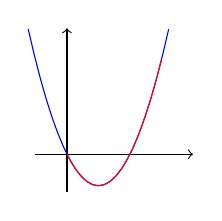
\begin{tikzpicture}[scale=0.4]
		\draw[->] (-1, 0) -- (4, 0);
		\draw[->] (0, -1.2) -- (0, 4);
		\draw[blue, domain=-1.23:3.23] plot(\x, \x * \x - 2 * \x);
		\draw[red, domain=0:3] plot(\x, \x * \x - 2 * \x);
	\end{tikzpicture}
\end{minipage}

\subsection[复合]{复合(无图)}
但是有些函数的图像你可是画不出来的,比如$y=4^x-2^{x+1}+1$。那就应该使用复合函数求值域的方法了。

如果一个函数$y=f(x)$可复合成$t=g(x)$和$y=f(t)$,那么可先求$g(x)$的值域,记为$A$。然后以$A$为定义域求$f(t)$的值域
(其中$f$、$g$均可作图)。

\subsubsection{分式复合}


\subsection{非复合}
上面介绍了这么多的复合函数求值域的方法,虽然多,但不可能用在所有函数上。那这些无法复合函数我们就不能求出它们的值域。

但是我们非常的幸运,拿到了一个单调函数(或者说函数在定义域内单调),那还是有办法的,直接代端点就可以了。

\begin{example}
	求$y=(\frac{1}{2})^x+(\frac{1}{3})^x,x\in(-\infty,2]$的值域
\end{example}
\begin{proof}[解]
	由题意得,函数单调递减。
	
	$\therefore y\in[\frac{13}{36},+\infty)$
\end{proof}

\section{何为数理分析}
在前面的小节中,我们学会了求解三样东西:不等式、值域和方程。它们是数理分析的主要手段。

数理分析的基本思想:等式(即方程)用掉一个等式,可以减少一个未知数的个数(即消元),最终获得只含一个未知数的等式、代数式或不等式。

所谓的数理分析即:在正式计算前的一种预测,即将多于等式的未知数全部用掉后,在最终一个等式的情况下,未知数还剩几个:

\begin{desclist}
	\item[若只剩一个未知数] 可求值
	\item[若剩两个未知数] 则可求范围
	\item[若剩超过两个未知数] 则此题还有变数(可能是条件还没有找到,可能需要等待一个巧合,可能是双变量等等)
\end{desclist}
